% Bien dich tu thu muc docs/report/lab3:
% pdflatex -interaction=nonstopmode -halt-on-error vmprint.tex
% Chay hai lan de cap nhat tham chieu.
\documentclass[a4paper]{article}
\usepackage[utf8]{vntex}
\usepackage{a4wide,amsmath,amssymb,array,booktabs,tabularx}
\usepackage{graphicx,fancyhdr,float,caption}
\usepackage{listings,xcolor}
\usepackage[most]{tcolorbox}
\usepackage[shortlabels]{enumitem}
\usepackage{indentfirst}
\usepackage{hyperref}

\renewcommand{\baselinestretch}{1.5}
\renewcommand{\tablename}{Bảng}
\renewcommand{\figurename}{Hình}
\renewcommand{\refname}{Tài liệu tham khảo}
\renewcommand{\lstlistingname}{Đoạn mã}
\setlength{\headheight}{40pt}
\setlength{\emergencystretch}{2em}
\setlength{\tabcolsep}{5pt}
\renewcommand{\arraystretch}{1.25}

\definecolor{codegreen}{rgb}{0,0.6,0}
\definecolor{codegray}{rgb}{0.5,0.5,0.5}
\definecolor{codepurple}{rgb}{0.58,0,0.82}
\definecolor{backcolour}{rgb}{0.95,0.95,0.92}
\definecolor{termBG}{HTML}{0C1C23}
\definecolor{termWhite}{HTML}{F8F8F2}
\lstdefinestyle{mystyle}{
  language=C,
  backgroundcolor=\color{backcolour},
  commentstyle=\color{codegreen},
  keywordstyle=\color{magenta},
  numberstyle=\tiny\color{codegray},
  stringstyle=\color{codepurple},
  basicstyle=\linespread{1}\selectfont\ttfamily\footnotesize\color{black},
  numbers=left,numbersep=6pt,
  keepspaces=true,columns=fullflexible,
  showstringspaces=false,showtabs=false,
  breaklines=true,tabsize=2,frame=single,
  captionpos=b,aboveskip=8pt,belowskip=8pt
}
\lstdefinestyle{terminalstyle}{
  language={},
  basicstyle=\linespread{1}\selectfont\ttfamily\scriptsize\color{termWhite},
  backgroundcolor=\color{termBG},
  numbers=none,columns=fullflexible,keepspaces=true,
  showstringspaces=false,breaklines=true,
  frame=single,rulecolor=\color{termBG},framesep=5pt,
  aboveskip=8pt,belowskip=8pt
}
\lstset{style=mystyle}
\newtcbox{\code}{on line,arc=2pt,colback=gray!20,colframe=gray!20,
  boxrule=0pt,boxsep=0pt,left=2pt,right=2pt,top=1pt,bottom=1pt,
  fontupper=\ttfamily}
\hypersetup{colorlinks=true,linkcolor=black,citecolor=red,urlcolor=blue,
  pdftitle={Lab 03 - Page Table: vmprint},
  pdfauthor={Phuc-Khang Nguyen; Minh-Trong Pham; Trong-Nghia Hoang}}

\pagestyle{fancy}
\fancyhf{}
\fancyhead[L]{
  \color{black}
  \begin{tabular}{rl}
    \begin{picture}(25,15)(0,0)
      \put(0,-8){
\includegraphics[width=8mm,height=8mm]{../lab2/images/khtn.png}}
    \end{picture}&
    \begin{tabular}{l}
      \textbf{\ttfamily Ho Chi Minh University of Science - VNUHCM}\\
      \textbf{\ttfamily Faculty of Information Technology}
    \end{tabular}
  \end{tabular}
}
\fancyfoot[L]{\color{black}\scriptsize\ttfamily Operating Systems -- Lab 03: Page Table}
\fancyfoot[R]{\color{black}\scriptsize\ttfamily Page \thepage}
\renewcommand{\headrulewidth}{0.3pt}
\renewcommand{\footrulewidth}{0.3pt}

\begin{document}
\renewcommand{\refname}{Tài liệu tham khảo}

\section{vmprint(): In bảng trang}

Trong hệ điều hành xv6, mỗi tiến trình sử dụng một bảng trang để ánh xạ
địa chỉ ảo sang địa chỉ vật lý. Với cơ chế Sv39, cấu trúc này được tổ chức
thành cây gồm ba cấp: L2, L1 và L0. Để quan sát các ánh xạ và quyền truy
cập của tiến trình, nhóm triển khai hàm \code{vmprint(pagetable\_t pagetable)}
tại \texttt{kernel/vm.c}. Hàm nhận vào bảng trang gốc, duyệt các PTE hợp lệ
và in ra chỉ số mục, giá trị PTE cùng địa chỉ vật lý đích theo định dạng
phân tầng của đề bài \cite{labguide,mitpgtbl}.

\subsection{Triển khai}

\paragraph*{Tổ chức thành hai hàm:}
Nhóm chia quá trình xử lý thành hàm giao diện \code{vmprint()} và hàm
trợ giúp đệ quy \code{vmprintwalk(pagetable\_t pagetable, int depth)}.
Hàm \code{vmprint()} giữ đúng giao diện một tham số mà đề bài yêu cầu,
in địa chỉ bảng gốc và khởi động quá trình duyệt với \code{depth = 1}.
Hàm \code{vmprintwalk()} nhận thêm độ sâu để xác định số nhóm dấu
\texttt{..} cần in khi đi xuống từng cấp của cây.

Hàm \code{vmprint()} được kernel gọi trực tiếp, không phải một system
call mới. Nhóm khai báo \code{void vmprint(pagetable\_t);} trong
\texttt{kernel/defs.h} để \texttt{kernel/exec.c} gọi được hàm đã định
nghĩa tại \texttt{kernel/vm.c}. Hàm phụ được khai báo \code{static}
vì chỉ sử dụng nội bộ trong tệp này. Cách tổ chức trên giữ giao diện
bên ngoài đơn giản, trong khi độ sâu được truyền riêng qua từng
lần gọi đệ quy.


\paragraph*{Cấu trúc bảng trang và các cờ PTE:}
Mỗi bảng trang ở một cấp chiếm $4096$ byte và chứa $512$ PTE, mỗi PTE
dài $8$ byte. Kiểu \code{pagetable\_t} được định nghĩa là con trỏ tới
các phần tử $64$ bit, còn \code{pte\_t} là một số nguyên $64$ bit.
Do đó, phép gán \code{pte\_t pte = pagetable[i];} đọc toàn bộ giá trị
của PTE thứ \code{i} trong bảng hiện tại \cite{localsource}.

Một PTE chứa trường số hiệu trang vật lý (PPN -- Physical Page Number)
và các bit cờ; PTE không lưu tên vùng nhớ như code, data hay stack.
Địa chỉ vật lý đích được suy ra từ PPN, còn vai trò của trang được xác
định bằng vị trí ánh xạ và cách kernel thiết lập trang đó.
Các cờ được đặt trong $10$ bit thấp, bố trí như sau \cite{riscvspec}:

\begin{center}
\small
\begin{tabular}{c|ccccccccc}
\toprule
Vị trí bit & $9$--$8$ & $7$ & $6$ & $5$ & $4$ & $3$ & $2$ & $1$ & $0$\\
Tên trường & RSW & D & A & G & U & X & W & R & V\\
\bottomrule
\end{tabular}
\end{center}

Trong đó, V cho biết mục có hợp lệ hay không; R, W, X lần lượt biểu
diễn quyền đọc, ghi và thực thi; U cho biết user mode có được truy cập
theo các quyền đó hay không. G đánh dấu ánh xạ global; A ghi nhận việc
truy cập; D ghi nhận việc ghi; hai bit RSW dành cho phần mềm hệ thống.
Để kiểm tra một cờ, nhóm dùng phép AND giữa giá trị PTE với mặt nạ
tương ứng. Kết quả khác $0$ có nghĩa là cờ đang bật, không nhất thiết
phải bằng $1$.


\paragraph*{Duyệt và bỏ qua các mục không hợp lệ:}
Tại mỗi lần gọi, \code{vmprintwalk()} nhận địa chỉ bảng đang xét cùng
\code{depth}, rồi duyệt lần lượt các chỉ số từ $0$ đến $511$.
Sau khi đọc một PTE, hàm kiểm tra \code{(pte \& PTE\_V) == 0}.
Nếu điều kiện đúng, hàm thực hiện \code{continue} để chuyển sang mục
kế tiếp. Nhờ đó, đầu ra chỉ chứa các ánh xạ hợp lệ; những mục trống
không được in và cũng không được dùng để đi xuống bảng con.

\paragraph*{Trích xuất địa chỉ vật lý:}
Với mỗi PTE hợp lệ, nhóm sử dụng macro \code{PTE2PA} được định nghĩa
trong \texttt{kernel/riscv.h} để xác định địa chỉ vật lý đích và lưu
vào biến \code{pa}. Trong các PTE do xv6 tạo ở bài này, các bit cao
dành riêng bằng $0$. Trước hết, giá trị PTE được dịch phải $10$ bit
để loại bỏ phần cờ và thu được số hiệu trang vật lý PPN. Sau đó,
giá trị này được dịch trái $12$ bit, tương đương nhân với kích thước
trang $4096$ byte, để tính địa chỉ bắt đầu của trang vật lý. Địa chỉ
thu được có $12$ bit thấp bằng $0$ vì trang được căn theo ranh giới
$4$ KB. Như vậy, quá trình này loại bỏ các cờ để trích xuất địa chỉ;
nếu chỉ muốn lấy riêng $10$ bit cờ, nhóm sử dụng phép AND với mặt nạ
\texttt{0x3FF}.

\paragraph*{Phân biệt bảng trang con và PTE lá:}
Sau khi xác nhận V bằng $1$, nhóm kiểm tra đồng thời ba bit R, W, X.
Đối với các PTE hợp lệ mà xv6 tạo trong bài này, nếu cả ba bit đều
bằng $0$ thì \code{pa} trỏ tới một bảng trang cấp dưới. Nếu có ít nhất
một bit được bật thì mục đó là PTE lá, trỏ tới trang vật lý được ánh
xạ và không cần đệ quy tiếp. Bit U không quyết định một PTE có phải
là lá hay không: trang bảo vệ stack và TRAPFRAME vẫn là các trang lá
mặc dù không bật U.

Nhóm sử dụng duyệt theo chiều sâu (DFS), in PTE hiện tại trước rồi
mới duyệt bảng con của nó. Khi đi xuống, lời gọi
\code{vmprintwalk((pagetable\_t)pa, depth + 1)} tăng độ sâu một đơn vị.
Sau khi duyệt hết bảng con, hàm quay về bảng cha để xét chỉ số kế
tiếp. Thứ tự này giữ các mục của cùng một nhánh nằm liền nhau trong
đầu ra. Cách duyệt được tham khảo từ \code{freewalk()}, nhưng
\code{vmprintwalk()} chỉ đọc và in, không sửa PTE hoặc giải phóng
bất kỳ trang nhớ nào.

Việc ép \code{pa} sang \code{pagetable\_t} rồi đọc bảng con phù hợp
với xv6 vì vùng RAM này được kernel ánh xạ trực tiếp: địa chỉ ảo
kernel bằng địa chỉ vật lý tương ứng. Điều này không có nghĩa là
kernel luôn có thể giải tham chiếu trực tiếp mọi địa chỉ ảo của user.

\paragraph*{Định dạng độ sâu và thông tin đầu ra:}
Biến \code{depth} là số nhóm dấu \texttt{..}, không phải số hiệu cấp
Sv39. Nhóm khởi tạo \code{depth = 1} ở L2, tăng thành $2$ ở L1 và
thành $3$ ở L0. Trước hết, hàm in một nhóm \texttt{..}; vòng lặp
\code{for(int j = 1; j < depth; j++)} in thêm \code{depth - 1} nhóm
\texttt{ ..}. Vì vậy, các tiền tố lần lượt là \texttt{..},
\texttt{.. ..} và \texttt{.. .. ..}.

Sau tiền tố, hàm in chỉ số \code{i}, giá trị \code{pte} và địa chỉ
\code{pa}. Chỉ số \code{i} là vị trí trong bảng hiện tại, không phải
số trang ảo của toàn bộ tiến trình; cùng một chỉ số có thể xuất hiện
ở nhiều bảng khác nhau. Định dạng \texttt{\%p} của \code{printf()}
trong xv6 in tiền tố \texttt{0x} và đủ $16$ chữ số hex. Các phép ép
\code{(void*)pte} và \code{(void*)pa} phục vụ lời gọi in, không đọc
nội dung tại địa chỉ đó.


\paragraph*{Tích hợp vào quá trình nạp chương trình:}
Cuối cùng, tại \texttt{kernel/exec.c}, nhóm thêm lời gọi ngay trước
\code{return argc;} sau khi bảng trang mới đã được gán cho tiến trình:

\begin{lstlisting}[numbers=none]
if(p->pid == 1)
  vmprint(p->pagetable);
\end{lstlisting}

Điều kiện PID bằng $1$ giới hạn việc in cho tiến trình đầu tiên.
Trong quá trình khởi động thông thường, kernel in bảng trang ngay
sau khi nạp xong chương trình \texttt{init}, trước khi chương trình
này bắt đầu chạy ở user mode. Về bản chất, hàm in cấu trúc ánh xạ;
nó không in nội dung mã lệnh hoặc dữ liệu nằm trong các trang lá.

\subsection{Kiểm thử}

Sau khi hoàn tất quá trình triển khai, nhóm kiểm tra hàm
\texttt{vmprint()} trên QEMU nhằm đánh giá định dạng đầu ra, cách
phân tầng bảng trang và khả năng hoạt động của hệ thống sau khi in
(Bảng~\ref{tab:vmprint_checks}).

\begin{table}[H]
\centering\small
\begin{tabularx}{\textwidth}{p{0.33\textwidth} X}
\toprule
\textbf{Kịch bản kiểm thử} & \textbf{Mục đích kiểm tra}\\
\midrule
Khởi động xv6 trên QEMU
 & Kiểm tra bảng trang của tiến trình đầu tiên được in sau khi nạp \texttt{init}, gồm địa chỉ gốc, chỉ số PTE, giá trị PTE và địa chỉ vật lý.\\
Đối chiếu cấu trúc đầu ra
 & Kiểm tra ba cấp thụt lề, bỏ qua PTE không hợp lệ, duyệt bảng con và dừng tại PTE lá.\\
\texttt{echo vmprint-ok}
 & Xác nhận shell tiếp tục nhận lệnh và trả về kết quả sau khi in bảng trang.\\
\bottomrule
\end{tabularx}
\caption{Các kịch bản kiểm thử tính năng in bảng trang}
\label{tab:vmprint_checks}
\end{table}

Kết quả thực nghiệm trên QEMU (Hình~\ref{fig:vmprint_result}) cho thấy:
\begin{itemize}[noitemsep,topsep=2pt]
\item \textbf{Cấu trúc phân tầng:} Đầu ra có $11$ PTE hợp lệ, gồm
$7$ PTE lá. Các mục L2, L1, L0 lần lượt có một, hai, ba nhóm dấu
\texttt{..}; địa chỉ \texttt{pa} khớp với giá trị trích xuất từ PTE.
\item \textbf{Nội dung các trang lá:} Ở nhánh địa chỉ thấp, mục $0$
chứa text/rodata (R, X, U); mục $1$ chứa data/BSS (R, W, U); mục $2$
là guard page (R, W, không có U); mục $3$ và $4$ là user stack
(R, W, U). Ở nhánh địa chỉ cao, mục $510$ là TRAPFRAME
(R, W, không có U), mục $511$ là TRAMPOLINE (R, X, không có U).
Tất cả các mục này đều bật V. Bản dựng kiểm tra có hai trang stack
và chưa ánh xạ USYSCALL.
\item \textbf{Hoạt động hệ thống:} Sau khi in, \texttt{init} khởi động
shell và lệnh \texttt{echo vmprint-ok} trả về đúng \texttt{vmprint-ok}.
\end{itemize}

\begin{figure}[H]
\centering
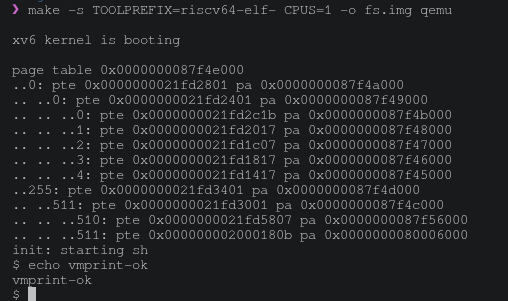
\includegraphics[width=0.85\textwidth]{images/vmprint-qemu.png}
\caption{Kết quả in bảng trang và thực thi lệnh kiểm tra trên QEMU}
\label{fig:vmprint_result}
\end{figure}

\begingroup
\small
\renewcommand{\baselinestretch}{1.1}\selectfont
\begin{thebibliography}{9}
\bibitem{labguide}
\textit{xv6 Lab 3 -- Page Table (Single-Page Scroll Guide)},
mục Yêu cầu, phần 4.2: In bảng trang. Tài liệu HTML cục bộ
\texttt{lab3-pagetable-guide.html} do thành viên cung cấp.

\bibitem{localsource}
Mã nguồn tại thời điểm viết báo cáo: \texttt{kernel/vm.c},
\texttt{kernel/riscv.h}, \texttt{kernel/defs.h},
\texttt{kernel/exec.c}, \texttt{kernel/proc.c},
\texttt{kernel/memlayout.h}, \texttt{kernel/param.h}
và \texttt{user/user.ld}.

\bibitem{mitpgtbl}
MIT PDOS, \textit{Lab: page tables}, mục ``Print a page table''.
\url{https://pdos.csail.mit.edu/6.1810/2022/labs/pgtbl.html}.

\bibitem{riscvspec}
RISC-V International, \textit{The RISC-V Instruction Set Manual,
Volume II: Privileged Architecture}, mục Supervisor-Level ISA,
các trường PTE và cơ chế Sv39.
\url{https://docs.riscv.org/reference/isa/priv/supervisor.html}.
\end{thebibliography}
\endgroup

\end{document}
